% !TeX root = ../../../book.tex
\subsection{多米诺与密铺} \label{sec:section2.4.1}

下面的示例比前两个示例稍微复杂一些。我们最终仍将证明某个数值公式,但问题显然比仅仅操纵代数表达式更加直观。此外,我们会在开始步骤中注意到一个有趣的``问题'',即我们必须解决几个``小案例'',然后才能推广我们的方法。这将是我们首次考虑如何泛化归纳技术使其适应其他情况。

我们要回答的问题可以表述如下:

\begin{quote}
    给定一个 $2 \times n$ 的正方形棋盘,有多少种不同的方式可以用多米诺骨牌平铺该棋盘?平铺必须让每个正方形都被一块——且只有一块——多米诺骨牌覆盖。
\end{quote}
例如,以下是正确的密铺

\begin{center}
    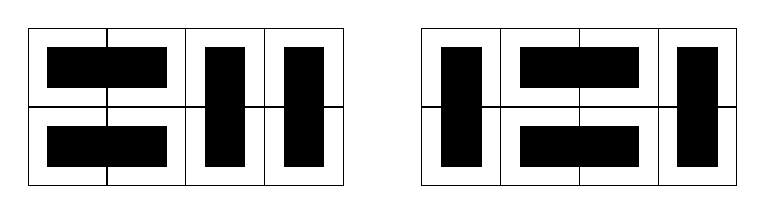
\begin{tikzpicture}[x=1.0cm, y=1.0cm]
        \foreach \y in {0,1} {
            \foreach \x in {0,...,3} {
                \draw (0+\x ,0+\y) rectangle ++ (1,1);
            }
        }

        \draw[fill, black] (0.25 ,0.25) rectangle ++ (1.5,0.5);
        \draw[fill, black] (0.25 ,1.25) rectangle ++ (1.5,0.5);
        \draw[fill, black] (2.25 ,0.25) rectangle ++ (0.5,1.5);
        \draw[fill, black] (3.25 ,0.25) rectangle ++ (0.5,1.5);

        \foreach \y in {0,1} {
            \foreach \x in {0,...,3} {
                \draw (5+\x ,0+\y) rectangle ++ (1,1);
            }
        }

        \draw[fill, black] (5+1.25 ,0.25) rectangle ++ (1.5,0.5);
        \draw[fill, black] (5+1.25 ,1.25) rectangle ++ (1.5,0.5);
        \draw[fill, black] (5+0.25 ,0.25) rectangle ++ (0.5,1.5);
        \draw[fill, black] (5+3.25 ,0.25) rectangle ++ (0.5,1.5);
    \end{tikzpicture}
\end{center}
而以下\emph{不}是正确的密铺

\begin{center}
    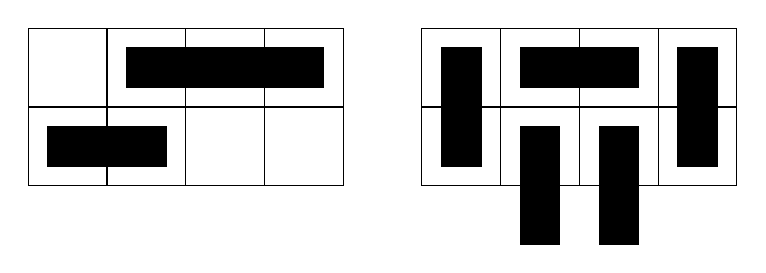
\begin{tikzpicture}[x=1.0cm, y=1.0cm]
        \foreach \y in {0,1} {
            \foreach \x in {0,...,3} {
                \draw (0+\x ,0+\y) rectangle ++ (1,1);
            }
        }

        \draw[fill, black] (0.25 ,0.25) rectangle ++ (1.5,0.5);
        \draw[fill, black] (1.25 ,1.25) rectangle ++ (1.5,0.5);
        \draw[fill, black] (2.25 ,1.25) rectangle ++ (1.5,0.5);

        \foreach \y in {0,1} {
            \foreach \x in {0,...,3} {
                \draw (5+\x ,0+\y) rectangle ++ (1,1);
            }
        }

        \draw[fill, black] (5+1.25 ,1.25) rectangle ++ (1.5,0.5);
        \draw[fill, black] (5+1.25 ,-0.75) rectangle ++ (0.5,1.5);
        \draw[fill, black] (5+2.25 ,-0.75) rectangle ++ (0.5,1.5);
        \draw[fill, black] (5+0.25 ,0.25) rectangle ++ (0.5,1.5);
        \draw[fill, black] (5+3.25 ,0.25) rectangle ++ (0.5,1.5);
    \end{tikzpicture}
\end{center}

和以前一样,让我们查看前几种情况(其中 $n = 1, 2, 3$ 等),看看我们是否能发现任何模式。在继续阅读之前,尝试自己解决该问题!

当 $n = 1$ 时,我们有一个与多米诺骨牌形状完全相同的棋盘,因此肯定只有一种方法可以密铺。让我们使用符号 $T(n)$ 来表示 $2 \times n$ 棋盘上的密铺数量。因此,$T(1) = 1$。

\begin{center}
    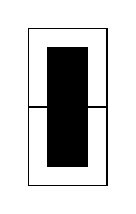
\begin{tikzpicture}[x=1.0cm, y=1.0cm]
        \draw (0,0) rectangle ++ (1,1);
        \draw (0,1) rectangle ++ (1,1);
        \draw[fill, black] (0.25 ,0.25) rectangle ++ (0.5,1.5);
    \end{tikzpicture}
\end{center}
当 $n = 2$ 时,我们有一个 $2 \times 2$ 棋盘。由于棋盘的方向很重要,因此我们有以下两种不同的密铺。因此,$T(2) = 2$。

\begin{center}
    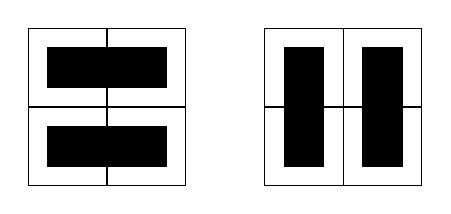
\begin{tikzpicture}[x=1.0cm, y=1.0cm]
        \foreach \y in {0,1} {
            \foreach \x in {0,1} {
                \draw (0+\x ,0+\y) rectangle ++ (1,1);
            }
        }

        \draw[fill, black] (0.25 ,0.25) rectangle ++ (1.5,0.5);
        \draw[fill, black] (0.25 ,1.25) rectangle ++ (1.5,0.5);

        \foreach \y in {0,1} {
            \foreach \x in {0,1} {
                \draw (3+\x ,0+\y) rectangle ++ (1,1);
            }
        }

        \draw[fill, black] (3+0.25 ,0.25) rectangle ++ (0.5,1.5);
        \draw[fill, black] (3+1.25 ,0.25) rectangle ++ (0.5,1.5);
    \end{tikzpicture}
\end{center}
当 $n = 3$ 时呢?同样地,我们可以手动枚举这些密铺,并确保没有遗漏任何一个。我们看到 $T(3) = 3$。

\begin{center}
    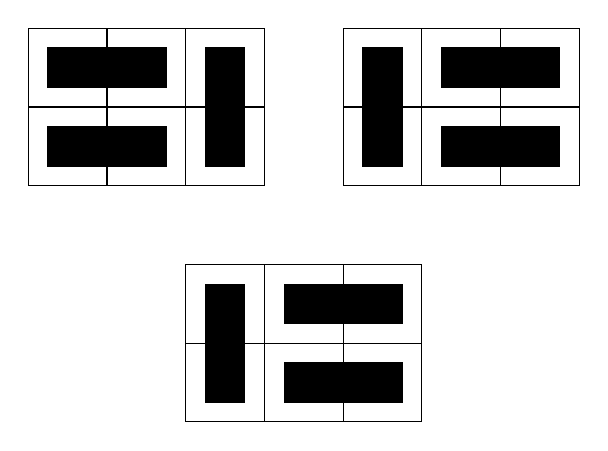
\begin{tikzpicture}[x=1.0cm, y=1.0cm]
        \foreach \y in {0,1} {
            \foreach \x in {0,1,2} {
                \draw (0+\x ,0+\y) rectangle ++ (1,1);
            }
        }

        \draw[fill, black] (0.25 ,0.25) rectangle ++ (1.5,0.5);
        \draw[fill, black] (0.25 ,1.25) rectangle ++ (1.5,0.5);
        \draw[fill, black] (2.25 ,0.25) rectangle ++ (0.5,1.5);

        \foreach \y in {0,1} {
            \foreach \x in {0,1,2} {
                \draw (4+\x ,0+\y) rectangle ++ (1,1);
            }
        }

        \draw[fill, black] (4+1.25 ,0.25) rectangle ++ (1.5,0.5);
        \draw[fill, black] (4+1.25 ,1.25) rectangle ++ (1.5,0.5);
        \draw[fill, black] (4+0.25 ,0.25) rectangle ++ (0.5,1.5);

        \foreach \y in {0,1} {
            \foreach \x in {0,1,2} {
                \draw (2+\x ,-3+\y) rectangle ++ (1,1);
            }
        }

        \draw[fill, black] (2+1.25 ,-3+0.25) rectangle ++ (1.5,0.5);
        \draw[fill, black] (2+1.25 ,-3+1.25) rectangle ++ (1.5,0.5);
        \draw[fill, black] (2+0.25 ,-3+0.25) rectangle ++ (0.5,1.5);
    \end{tikzpicture}
\end{center}
好的,再看一种情况,当 $n=4$ 时,我们看到 $T(4)=5$。

\begin{center}
    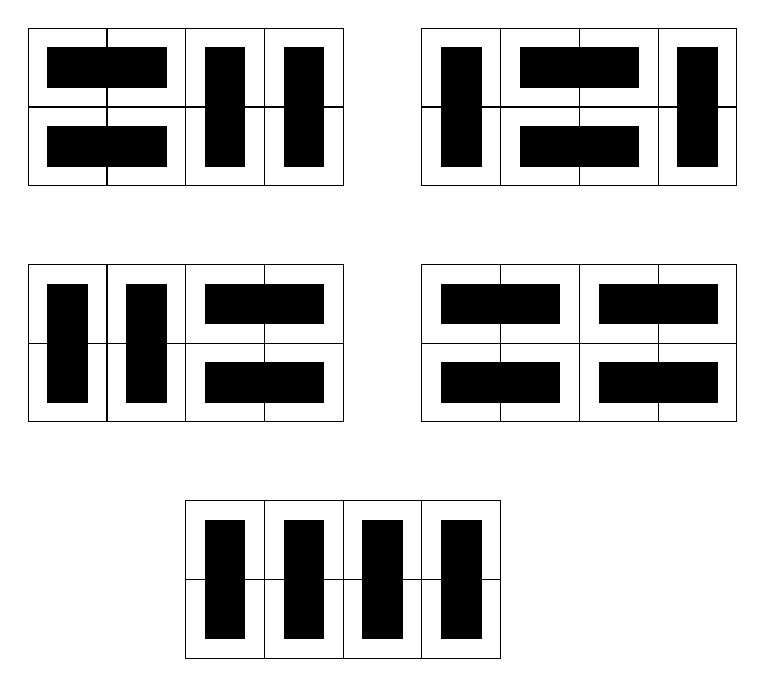
\begin{tikzpicture}[x=1.0cm, y=1.0cm]
        \foreach \y in {0,1} {
            \foreach \x in {0,...,3} {
                \draw (0+\x ,0+\y) rectangle ++ (1,1);
            }
        }

        \draw[fill, black] (0.25 ,0.25) rectangle ++ (1.5,0.5);
        \draw[fill, black] (0.25 ,1.25) rectangle ++ (1.5,0.5);
        \draw[fill, black] (2.25 ,0.25) rectangle ++ (0.5,1.5);
        \draw[fill, black] (3.25 ,0.25) rectangle ++ (0.5,1.5);

        \foreach \y in {0,1} {
            \foreach \x in {0,...,3} {
                \draw (5+\x ,0+\y) rectangle ++ (1,1);
            }
        }

        \draw[fill, black] (5+1.25 ,0.25) rectangle ++ (1.5,0.5);
        \draw[fill, black] (5+1.25 ,1.25) rectangle ++ (1.5,0.5);
        \draw[fill, black] (5+0.25 ,0.25) rectangle ++ (0.5,1.5);
        \draw[fill, black] (5+3.25 ,0.25) rectangle ++ (0.5,1.5);

        \foreach \y in {0,1} {
            \foreach \x in {0,...,3} {
                \draw (0+\x ,-3+\y) rectangle ++ (1,1);
            }
        }

        \draw[fill, black] (2.25 ,-3+0.25) rectangle ++ (1.5,0.5);
        \draw[fill, black] (2.25 ,-3+1.25) rectangle ++ (1.5,0.5);
        \draw[fill, black] (0.25 ,-3+0.25) rectangle ++ (0.5,1.5);
        \draw[fill, black] (1.25 ,-3+0.25) rectangle ++ (0.5,1.5);

        \foreach \y in {0,1} {
            \foreach \x in {0,...,3} {
                \draw (5+\x ,-3+\y) rectangle ++ (1,1);
            }
        }

        \draw[fill, black] (5+2.25 ,-3+0.25) rectangle ++ (1.5,0.5);
        \draw[fill, black] (5+2.25 ,-3+1.25) rectangle ++ (1.5,0.5);
        \draw[fill, black] (5+0.25 ,-3+0.25) rectangle ++ (1.5,0.5);
        \draw[fill, black] (5+0.25 ,-3+1.25) rectangle ++ (1.5,0.5);

        \foreach \y in {0,1} {
            \foreach \x in {0,...,3} {
                \draw (2+\x ,-6+\y) rectangle ++ (1,1);
            }
        }

        \draw[fill, black] (2+0.25 ,-6+0.25) rectangle ++ (0.5,1.5);
        \draw[fill, black] (2+1.25 ,-6+0.25) rectangle ++ (0.5,1.5);
        \draw[fill, black] (2+2.25 ,-6+0.25) rectangle ++ (0.5,1.5);
        \draw[fill, black] (2+3.25 ,-6+0.25) rectangle ++ (0.5,1.5);
    \end{tikzpicture}
\end{center}

我们现在可以开始寻找模式了吗?找到更大棋盘的密铺会很繁琐!让我们考虑一下如何利用 $T(1) = 1$ 的事实来推断出有关 $T(2)$ 的信息……等一下……做不到,对吧?这两个案例有本质的区别。具体来说,由于多米诺骨牌的大小为 $2 \times 1$,因此我们仅向棋盘中添加一行这一事实对我们没有帮助。

好吧,那么我们考虑 $n = 3$。我们可以利用 $T(2) = 2$ 这个事实吗?在这种情况下,答案是肯定的!知道 $2 \times 2$ 棋盘有两个密铺,无需太多思考,我们可以立即构建 $2 \times 3$ 棋盘的两个平铺。具体来说,我们可以将\emph{垂直多米诺骨牌添加}到之前的每一个密铺中。但我们知道 $T(3) = 3$。第三个密铺从何而来?再次查看该密铺,以及它与其他两个密铺的比较。在第三个密铺中,右侧的多米诺骨牌是水平的,而不是其他两种密铺中的垂直多米诺骨牌。如果我们移除这两个平行的水平多米诺骨牌,我们就会得到 $n = 1$ 时的情况。换句话说,我们可以通过在右侧\emph{添加一个由两个水平多米诺骨牌组成的正方形}来构建 $2 \times 3$ 棋盘的密铺。总的来说,我们已经用较小尺寸的棋盘(即 $2 \times 2$ 和 $2 \times 1$)描述了 $2 \times 3$ 棋盘的所有密铺:

\begin{center}
    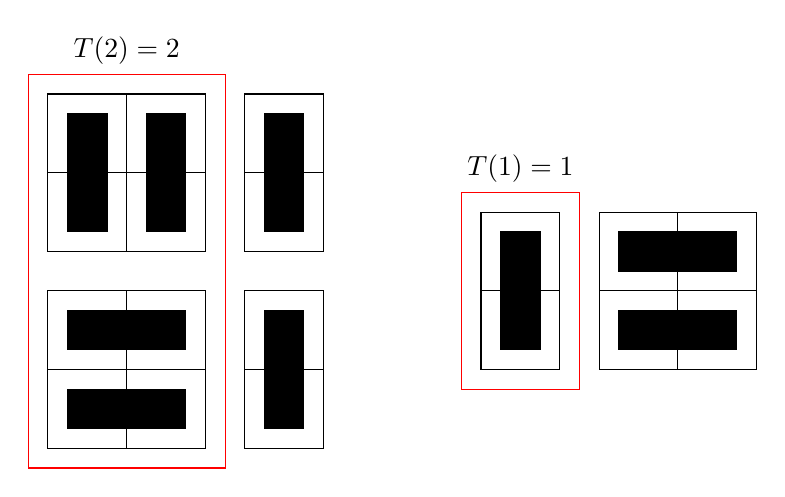
\begin{tikzpicture}[x=1.0cm, y=1.0cm]
        \foreach \g in {0, 2.5} {
            \foreach \y in {0,1} {
                \foreach \x in {0,1} {
                    \draw (0+\x ,0+\y+\g) rectangle ++ (1,1);
                }
            }
            \draw (2.5,0+\g) rectangle ++ (1,1);
            \draw (2.5,1+\g) rectangle ++ (1,1);
            \draw[fill, black] (2.75 ,0.25+\g) rectangle ++ (0.5,1.5);
        }

        \draw[fill, black] (0.25 ,0.25) rectangle ++ (1.5,0.5);
        \draw[fill, black] (0.25 ,1.25) rectangle ++ (1.5,0.5);

        \draw[fill, black] (0.25 ,2.5+0.25) rectangle ++ (0.5,1.5);
        \draw[fill, black] (1.25 ,2.5+0.25) rectangle ++ (0.5,1.5);

        \draw[red] (-0.25, -0.25) rectangle ++(2.5, 5);
        \path (-0.25,4.75) --  (2.25,4.75) node[midway,above,black] {$T(2)=2$};

        \draw (5.5,1) rectangle ++ (1,1);
        \draw (5.5,2) rectangle ++ (1,1);
        \draw[fill, black] (5.75 ,1.25) rectangle ++ (0.5,1.5);
        \draw[red] (5.25, 0.75) rectangle ++(1.5, 2.5);
        \path (5.25,3.25) --  (6.75,3.25) node[midway,above,black] {$T(1)=1$};

        \foreach \y in {0,1} {
            \foreach \x in {0,1} {
                \draw (7+\x ,1+\y) rectangle ++ (1,1);
            }
        }
        \draw[fill, black] (7.25 ,1.25) rectangle ++ (1.5,0.5);
        \draw[fill, black] (7.25 ,2.25) rectangle ++ (1.5,0.5);

    \end{tikzpicture}
\end{center}
\[T(3) = 3 = 2 + 1 = T(2) + T(1)\]

现在你可能会看出模式来!我们再看一下当 $n = 4$ 时会发生什么,我们将垂直多米诺骨牌添加到构成 $T(3)$ 的每一个密铺中,或者将两个水平多米诺骨牌添加到构成 $T(2)$ 的每一个密铺中,以此得到 $T(4)$ 的\emph{所有}密铺:

\begin{center}
    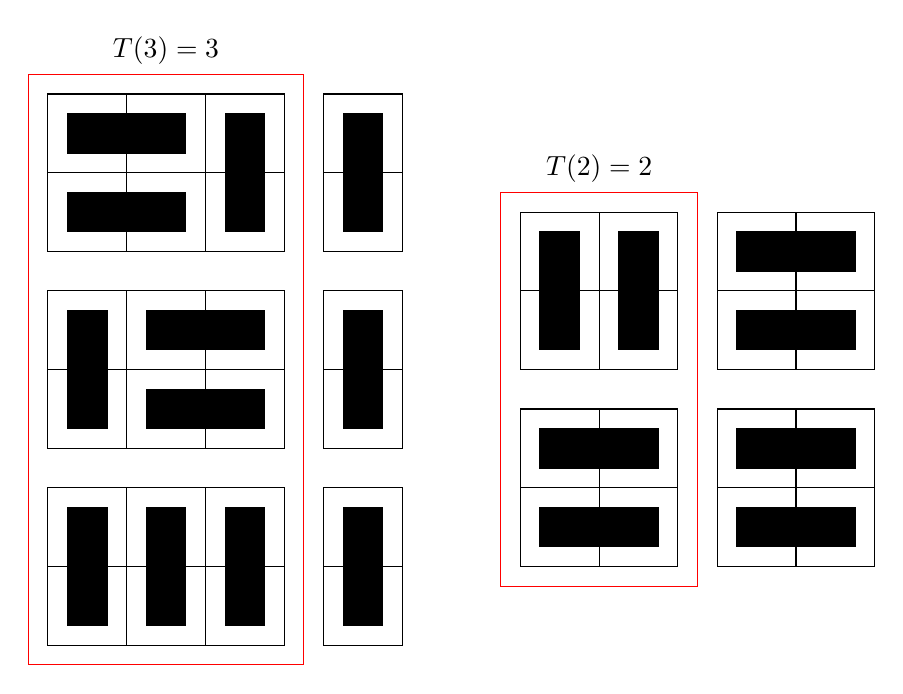
\begin{tikzpicture}[x=1.0cm, y=1.0cm]
        \foreach \g in {0, 2.5, 5} {
            \foreach \y in {0,1} {
                \foreach \x in {0,1,2} {
                    \draw (0+\x ,0+\y+\g) rectangle ++ (1,1);
                }
            }

            \draw (3.5,\g+0) rectangle ++ (1,1);
            \draw (3.5,\g+1) rectangle ++ (1,1);
            \draw[fill, black] (3.75 ,\g+0.25) rectangle ++ (0.5,1.5);
        }
        \draw[fill, black] (0.25 ,0.25) rectangle ++ (0.5,1.5);
        \draw[fill, black] (1.25 ,0.25) rectangle ++ (0.5,1.5);
        \draw[fill, black] (2.25 ,0.25) rectangle ++ (0.5,1.5);

        \draw[fill, black] (0.25 ,2.75) rectangle ++ (0.5,1.5);
        \draw[fill, black] (1.25 ,2.75) rectangle ++ (1.5,0.5);
        \draw[fill, black] (1.25 ,3.75) rectangle ++ (1.5,0.5);

        \draw[fill, black] (2.25 ,5.25) rectangle ++ (0.5,1.5);
        \draw[fill, black] (0.25 ,5.25) rectangle ++ (1.5,0.5);
        \draw[fill, black] (0.25 ,6.25) rectangle ++ (1.5,0.5);

        \draw[red] (-0.25, -0.25) rectangle ++(3.5, 7.5);
        \path (-0.25,7.25) --  (3.25,7.25) node[midway,above,black] {$T(3)=3$};


        \foreach \g in {0, 2.5} {
            \foreach \y in {0,1} {
                \foreach \x in {0,1} {
                    \draw (6+\x ,1+\y+\g) rectangle ++ (1,1);
                }
            }
            \foreach \y in {0,1} {
                \foreach \x in {0,1} {
                    \draw (8.5+\x ,1+\y+\g) rectangle ++ (1,1);
                }
                \draw[fill, black] (8.75 ,1.25+\g+\y) rectangle ++ (1.5,0.5);
            }
           
        }

        \draw[fill, black] (6.25 ,1.25) rectangle ++ (1.5,0.5);
        \draw[fill, black] (6.25 ,2.25) rectangle ++ (1.5,0.5);

        \draw[fill, black] (6.25 ,3.5+0.25) rectangle ++ (0.5,1.5);
        \draw[fill, black] (7.25 ,3.5+0.25) rectangle ++ (0.5,1.5);

        \draw[red] (5.75, 0.75) rectangle ++(2.5, 5);
        \path (5.75,5.75) --  (8.25,5.75) node[midway,above,black] {$T(2)=2$};
        
    \end{tikzpicture}
\end{center}
\[T(4) = 5 = 3 + 2 = T(3) + T(2)\]

另请注意,用这种方式不会产生重复的 $2 \times 4$ 密铺。(仔细想想为什么会这样。我们用一种什么方法表征两种密铺可以保证它们不重复?)有了这些信息,我们可以立即得出结论 $T(4) = T(3) + T(2)$。

此外,我们可以概括这样一个论点;$n = 4$ 没有什么特别的,对吧?对于任意特定的 $n$,我们可以只考虑所有可能的密铺,然后看看棋盘\emph{最右侧}发生的情况:要么有一个垂直多米诺骨牌(这意味着密铺来自 $2 \times (n - 1)$ 棋盘),要么有两个水平多米诺骨牌(这意味着密铺来自 $2 \times (n-2)$ 棋盘)。有了这个论点的支撑,对于所有有意义的 $n$ 值,我们可以得出如下结论:
\[T(n) = T(n - 1) + T(n - 2)\]
哪些 $n$ 值有意义?请记住,我们必须单独分析 $T(1)$ 和 $T(2)$;因此这个论点不适用于 $n=1$ 和 $n=2$,我们必须添加限制条件 $n \ge 3$ 才能使上面公式成立。

有了这些信息,只要有足够的时间,我们就可以轻松计算出任意 $n$ 值下的 $T(n)$。我们甚至可以相当容易地编写出计算机程序。然而,正是这种\emph{归纳}论证——我们注意到的模式以及我们对其发生原因的彻底描述——让我们首先得出了结论。这种情况下,每一项的值 $T(n)$ 取决于前\emph{两}项 $T(n-1)$ 和 $T(n-2)$ 的值。这在本章之前的例子中\emph{没有}出现过,它暗示了这里发生了更深层次的事情。你是否发现我们之前对归纳的定义以及多米诺骨牌的类比在这里不再适用?你会如何修正我们的类比来解释这种情况?思考一下这些问题,然后继续阅读。我们将在下一个示例之后更深入地讨论它们。

顺便一提,你是否注意到此示例的解有一些有趣的地方?你还知道其他类似的数列吗?想一想……
